
\section{Optimization strategies}\label{strategies}

This section outlines the mathematical derivations of the risk-based optimal portfolio strategies.
The final technical details, specific for each dispersion
measure, are left for next sections.


To better understand the various optimization strategies that will be explored in this paper, let us
look at Fig.~\ref{Frontiers_1_fig}.


\begin{figure}[H]
    \centering
    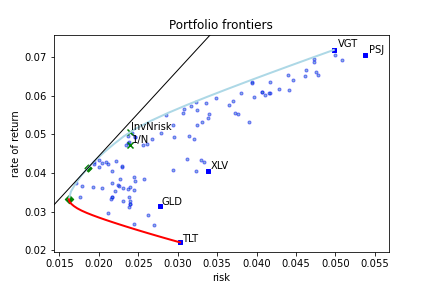
\includegraphics[width=.95\linewidth]{../figs/frontiers_1.png}
    \caption{Portfolio frontiers - expected rate of return vs. risk.}
    \label{Frontiers_1_fig}
\end{figure}

It is a generic example of portfolio frontiers. On the x-axis is the dispersion value (risk)
while on the y-axis is the expected rate of return. Given a set of financial assets, each point in this space represents a portfolio
composition. Several features are worth mentioning.


The upper blue line is the {\it efficient frontier}. This is the set of portfolios that have the highest expected rate
of return for a given risk value. These are the portfolios of interest for an investor.

The lower red line is the {\it inefficient frontier}. This is the set of portfolios that have the lowest expected rate
of return for a given risk value. Clearly, this family of portfolios are to be avoided by an investor.

The leftmost point, where the blue and red lines meet, is the {\it minimum risk portfolio}.
This is the portfolio with the smallest risk among all possible portfolios.
Investing in this class of portfolios is a relative common strategy among professional investors.

The black straight line, in the upper part of the plot, is tangent to the efficient frontier.
Its intersection with the y-axis (not shown in the plot) is at a level equal to the risk-free rate accessible to the investor.\footnote{In this example the risk-free rate was set to $0$.} The point of tangency along the efficient frontier (in our plot depicted by a green diamond)
is the so called {\it tangency portfolio} or {\it market portfolio}. This is the portfolio with the highest value of $\rho$-Sharpe ratio among all possible portfolios.
The $\rho$-Sharpe ratio is defined as
\begin{equation}
    \Sharpe = \frac{\RR-\mu_0}{\rho}, \label{ggg}
\end{equation}
where $\RR$ is the portfolio expected rate of return, $\mu_0$ is the risk-free rate accessible to the investor and
$\rho$ is the dispersion measure.\footnote{This is a generalization of the original Sharpe ratio introduced in 1966 by
William F. Sharpe \cite{Sharpe1966} as an  investment performance measure. In the original definition, $\rho$ is the
standard deviation (volatility) of the returns.}
Therefore, the portfolio that maximizes the $\rho$-Sharpe ratio is the portfolio with the highest expected excess rate of return (\ie\ above the risk-free rate) per unit of risk, $\rho$. This is a remarkable efficient portfolio often preferred by the investors.

The solid blue squares are the portfolios where the entire capital is allocated to a single component.
They are labeled by the market symbol of this portfolio component.\footnote{In our case the portfolio components are
5 ETF's: TLT, GLD, XLV, IHI and PSJ.} For short, we call them {\it single asset portfolios}.
Note that the rightmost point along the efficient frontiers is the single asset portfolio where the entire capital is invested in the portfolio component with the highest expected rate of return.
Similarly, the rightmost point along the inefficient frontier is the single asset portfolio where the entire
capital is invested in the portfolio component with the lowest expected rate of return.

All the points between the efficient (blue line) and inefficient (red line) frontiers are called {\it inefficient portfolios}.
For reference, in Fig.~\ref{Frontiers_1_fig} we depicted with small blue circles a random selection of them.
There are no valid portfolios outside the portfolio frontiers.

Among the inefficient portfolios, there is a remarkable one that has enjoined a lot of attention in the literature over the years.
This is the {\it equal weighted portfolio}.
As the name suggested, it has the weights equal to $1/N$, where $N$ is the number of portfolio components.
In Fig.~\ref{Frontiers_1_fig}, it is depicted by a green x labeled $1/N$.

On the efficient frontier, we have its correspondent. In our plot it is a green x with label InvNrisk.
This is the efficient portfolio that has the same risk as the equal weighted portfolio.

We stress that, in-sample both portfolios have the same risk while the expected rate of return is larger for InvNrisk
than for equal weighted portfolio.
However out-of-sample (especially for relatively short periods of observations) the equal weighted portfolio may outperform the InvNrisk.

\begin{figure}[H]
    \centering
    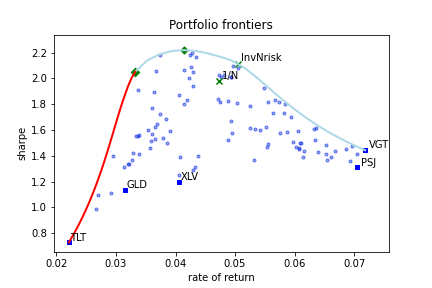
\includegraphics[width=.95\linewidth]{../figs/frontiers_2.png}
    \caption{Portfolio frontiers - $\rho$-Sharpe vs. expected rate of return.}
    \label{Frontiers_2_fig}
\end{figure}

Another way to visualize the portfolio frontiers is presented in Fig.~\ref{Frontiers_2_fig}.
It has the same information as Fig.~\ref{Frontiers_1_fig}, but now on the x-axis is the expected rate of return while on the y-axis is the $\rho$-Sharpe ratio.
We have preserved the color code and all the symbols from Fig.~\ref{Frontiers_1_fig}.
Note that in this representation the $\rho$-Sharpe portfolio is the maximum of the efficient frontier curve.

Figure~\ref{Frontiers_2_fig} gives a better understanding of portfolio efficiency in terms of expected excess return per unit of risk.

With these in mind, let's start to define the following optimization strategies. We have restricted our analysis to long-only positions in the portfolio
components.\footnote{This is a self-imposed restriction; in principle, it can be removed or replaced with specific position limits.}

\bigskip

\begin{description}
  \item[A.\label{OptRisk}]{\bf Minimization of risk for targeted expected rate of return value}

    This is the most common optimization strategy. It returns portfolio compositions along the efficient frontiers (the blue line in Figs.~\ref{Frontiers_1_fig} and
    \ref{Frontiers_2_fig}).
    Mathematically, it can be expressed as,

    \bigskip
    \noindent Minimize over $\{w_k\}_{k=1,\cdots,M}$
    \begin{subequations}\label{gg1}
    \begin{align}
        & g =  \rho\left(\sum_{k=1}^M w_k r_k \right), \label{gg1a} \\
        \st & \sum_{k=1}^M w_k \mu_k \ge \mu, \label{gg1b} \\
            & \sum_{k=1}^M w_k = 1, \label{gg1c} \\
            & w_k \ge 0. \label{gg1d}
    \end{align}
    \end{subequations}

    \noindent Here $g$ is the objective function, $\rho(\cdot)$ is the dispersion measure, $M$ is the number of portfolio component, $w_k$ are the portfolio
    weights, $r_k$ are the portfolio components rate of return
    with $\mu_k=\mE[r_k]$ their expectations and $\mu$ is the targeted portfolio expected rate of return.

    In general, if $\mu \leq \max_k\{\mu_k\}$ then the efficient portfolio expected rate of return is $\max\{\RR_{\min}, \mu \}$,
    where $\RR_{\min}$ is the minimum risk portfolio expected rate of return.
    Otherwise, the optimization problem from Eqs.~(\ref{gg1}) has no solution.

    Note that changing the direction of the inequality in Eq.~(\ref{gg1b}), the solution of the optimization problem
    will be a portfolio along the inefficient frontiers (the red line in Figs.~\ref{Frontiers_1_fig} and \ref{Frontiers_2_fig}). In this case,
    if $\mu \geq \min_k\{\mu_k\}$ then the portfolio expected rate of return is $\min\{\RR_{\min}, \mu \}$. Otherwise,
    there are no solutions.

    Equation~(\ref{gg1c}) is the weights normalization equation also called the {\it capital equation} and Eq.~(\ref{gg1d}) is the long-only positions constraint.
    These two types of equations will be present in all portfolio optimization algorithms.

  \item[B.\label{MinRisk}] {\bf Minimum risk portfolio}

    This is the efficient portfolio with the smallest risk, $\rho$.
    Mathematically, it is the solution of the above optimization problem without the constraint from Eq.~(\ref{gg1b}).

    We mentioned earlier that the optimization problem from Eqs.~(\ref{gg1}) will return the
    minimum risk portfolio if $\mu$ in Eq.~(\ref{gg1b}) is set to any value less than or equal to $\RR_{\min}$.
    In practice it is convenient to set $\mu=\min_k\{\mu_k\}$. Then, use {\it as is} the algorithm from Eqs.~(\ref{gg1}) to
    find the composition of minimum risk portfolio.
    This approach has been implemented in the \azapy\ package.

  \item[C.\label{TargetRisk}] {\bf Maximization of expected rate of return for targeted risk value}

    Another way to evaluate the efficient portfolios is to maximize the portfolio expected rate of return
    for a fixed risk vale. Mathematically this can be written as follows.

    \bigskip
    \noindent Maximize over $\{w_k\}_{j=k,\cdots,M}$
    \begin{subequations}\label{gg2}
    \begin{align}
        & g =  \sum_{k=1}^M w_k \mu_k, \label{gg2a} \\
        \st & \rho\left(\sum_{k=1}^M w_k r_k \right) = \rho_0, \label{gg2b} \\
            & \sum_{k=1}^M w_k = 1, \label{gg2c} \\
            & w_k \ge 0. \label{gg2d}
    \end{align}
    \end{subequations}

    \noindent Here $\rho_0$ is the targeted portfolio risk value.
    In general, it is unintuitive for an investor to specify outright a rational value for $\rho_0$.
    However, if $\rho_0$ is the risk value of a benchmark portfolio, then the maximization problem
    from Eqs.~(\ref{gg2}) becomes useful in computing an efficient portfolio with the same risk as the benchmark.

    An example is the efficient portfolio with the same risk as equal weighted portfolio.
    In Figs.~\ref{Frontiers_1_fig} and \ref{Frontiers_2_fig} this is the efficient portfolio depicted with green x and labeled InvNrisk.
    In general, given a dispersion measure, it is straightforward to evaluate the risk of equal weighted portfolio, $\rho_{\rm EWP}$.
    Then, the weights of InvNrisk portfolio are the solution of Eqs.~(\ref{gg2})
    for $\rho_0 = \rho_{\rm EWP}$. Given the popularity of this benchmark,
    the evaluation of InvNrisk efficient portfolio is explicitly implemented in the \azapy\ package.

  \item[D.\label{RiskAverse}] {\bf Maximization of expected rate of return for fixed risk-aversion factor}

    In this strategy the optimal portfolio weights maximize the quantity $\RR-\lambda\rho$,
    where \RR\ is the portfolio expected rate of return, $\rho$ is the dispersion measure,
    and $\lambda$ is the risk-aversion factor. $\lambda$ takes values between $0$ and $+\infty$.
    For $\lambda=0$, the optimal portfolio is the single asset portfolio where the entire capital is invested in the
    component with the highest expected rate of return.
    This is the rightmost point along the efficient frontier.
    For $\lambda=+\infty$, the optimal portfolio is the minimum risk portfolio, the leftmost point on the efficient frontier.
    Any other value for $\lambda$ will lead to an optimal portfolio along the efficient frontier.

    The maximization problem defining this strategy can be expressed as,

    \bigskip
    \noindent Maximize over $\{w_k\}_{k=1,\cdots,M}$
    \begin{subequations}\label{gg3}
    \begin{align}
        & g =  \sum_{k=1}^M w_k \mu_k - \lambda\rho\left(\sum_{k=1}^M w_k r_k \right), \label{gg3a} \\
        \st & \sum_{k=1}^M w_k = 1, \label{gg3b} \\
            & w_k \ge 0. \label{gg3c}
    \end{align}
    \end{subequations}

    \noindent It is unintuitive for an investor to specify outright a rational value for the risk-aversion factor $\lambda$.
    However, this optimization strategy may become useful if it is combined with a model to estimate the
    value of the risk-aversion factor based on the market conditions (\eg\ technical analysis, etc.).
    These risk-aversion models are beyond the scope of this paper.

    Note that the optimization problems from Eqs.~(\ref{gg1}), (\ref{gg2}) and (\ref{gg3}) are equivalent
    in the sense that they lead to the same efficient portfolios but under different parameterizations, \ie,
    \begin{quote}
    \begin{description}
        \item[$\mu$] - the expected rate of return in Eqs.~(\ref{gg1}),
        \item[$\rho_0$] - the risk targeted value in Eqs.~(\ref{gg2}),
        \item[$\lambda$] - the risk aversion factor in Eqs.~(\ref{gg3}).
    \end{description}
    \end{quote}
    From a numerical point of view, they have quite different implementations.


  \item[E.\label{MaxSharpe}] {\bf Maximization of the $\rho$-Sharpe ratio}

    Given a dispersion measure $\rho$, this is the portfolio with the highest value of $\rho$-Sharpe ratio,
    $\Sharpe$ from Eq.~(\ref{ggg}).
    It is the solution of the following optimization problem.

    \bigskip
    \noindent Maximize over $\{w_k\}_{k=1,\cdots,M}$
    \begin{subequations}\label{gg4}
    \begin{align}
        & g = \frac{ \sum_{k=1}^M w_k \mu_k - \mu_0}{\rho\left(\sum_{k=1}^M w_k r_k \right)}, \label{gg4a} \\
        \st & \sum_{k=1}^M w_k = 1, \label{gg4b} \\
            & w_k \ge 0. \label{gg4c}
    \end{align}
    \end{subequations}

    \noindent Depending on the actual mathematical structure of $\rho$, this optimization can be transformed into an
    LP, QP or SOCP problem. Formally, this procedure can be described as follows.

    {\it First step.} Introduce a new variable $t$ such that
    \begin{equation}
        \frac{1}{t} \geq \rho\left(\sum_{k=1}^M w_k r_k \right), \label{gg5}
    \end{equation}
    and the variable transformations $\bw_k = w_k t$. Then, the optimization problem from Eqs.~(\ref{gg4}) can be expressed as follows.

    \bigskip
    \noindent Maximize over $\{ \{\bw_k\}_{k=1,\cdots,M}, t\}$
    \begin{subequations}\label{gg6}
    \begin{align}
        & g =  \sum_{k=1}^M \bw_k \mu_k - \mu_0 t, \label{gg6a} \\
        \st & t\rho\left(\sum_{k=1}^M w_k r_k \right) \leq 1, \label{gg6b} \\
            & \sum_{k=1}^M \bw_k - t = 0, \label{gg6c} \\
            & \bw_k \ge 0, \label{gg6d} \\
            & t \ge 0. \label{gg6e}
    \end{align}
    \end{subequations}

    \noindent {\it Second step.} Rewrite Eq.~(\ref{gg6b}) in terms of $\{\bw_j\}_{j=1,\cdots,M}$ and $t$ as a linear or second order cone constraint.
    This will become evident in the next sections where we will deal with explicit expressions for
    $\rho$ functions.\footnote{If $\rho$ is a genuine dispersion measure (see \cite{MM}), then by definition it is positive homogeneous and
    so $t\rho\left(\sum_{k=1}^M w_k r_k \right)=\rho\left(\sum_{k=1}^M \bw_k r_k \right)$. However, writing Eq.~(\ref{gg6}) in terms of
    $\bw_k$ and $t$ only is possible for a larger class of functions $\rho$.}
    Finally, the actual weights can be recovered by dividing $\bw_j$ by $t$.

    This procedure is in the spirit of Charnes-Copper transformation \cite{Charnes} of linear fractional functional programming,
    now extended to SOCP problems.


  \item[F.\label{MinSharpe}] {\bf Minimization of the inverse $\rho$-Sharpe ratio}

    The minimization of the inverse of $\rho$-Sharpe ratio follows a similar procedure as above.
    It is described by the following optimization problem,

    \bigskip
    \noindent Minimize over $\{w_k\}_{k=1,\cdots,M}$
    \begin{subequations}\label{gg4:2}
    \begin{align}
        & g = \frac{\rho\left(\sum_{k=1}^M w_k r_k \right)}{ \sum_{k=1}^M w_k \mu_k - \mu_0}, \label{gg4a:2} \\
        \st & \sum_{k=1}^M w_k = 1, \label{gg4b:2} \\
            & w_k \ge 0. \label{gg4c:2}
    \end{align}
    \end{subequations}

    \noindent In this case the variable $t$ is defined as
    \begin{equation}
      \frac{1}{t} = \sum_{k=1}^M w_k \mu_k - \mu_0, \label{gg7}
    \end{equation}
    and the optimization problem from Eqs.~(\ref{gg4:2}) can be expressed as

    \bigskip
    \noindent Minimize over $\{\{\bw_j\}_{j=1,\cdots,M}, t\}$
    \begin{subequations}\label{gg8}
    \begin{align}
        & g = t \rho\left(\sum_{k=1}^M w_k r_k \right), \label{gg8a} \\
        \st & \sum_{k=1}^M \bw_k \mu_k - \mu_0 t = 1, \label{gg8b} \\
            & \sum_{k=1}^M \bw_k - t = 0, \label{gg8c} \\
            & \bw_k \ge 0, \label{gg8d} \\
            & t \ge 0. \label{gg8e}
    \end{align}
    \end{subequations}

    \noindent Again, the trick is to rewrite Eq.~(\ref{gg8a}) in terms of $\{\bw_k\}_{k=1,\cdots,M}$ and $t$ variables only.
    This will be made explicit in the next sections.
\end{description}

\noindent The two problems, maximization of $\rho$-Sharpe ratio and the minimization of inverse of $\rho$-Sharpe ratio, are logically
equivalent, and the solutions of Eqs.~(\ref{gg6}) and (\ref{gg8}) are the same. However, from a numerical
point of view their implementations can be quite different. In our experience both methods lead to numerical algorithms 
similar in speed and accuracy. For completeness, \azapy\ package implements both methods.


\BackToContents
